\subsection{qiskit and OpenQASM}
Even though the two circuits appear different, they are equivalent because the part of the second circuit that contains a CNOT gate surrounded by Hadamard gates is mathematically equivalent to a controlled-$Z$ gate. Since this transformation does not change the overall effect of the circuit on the qubits, both circuits perform the same computation and therefore produce the same final state and the same measurement result, as shown below.

\begin{lstlisting}[language=Python, caption={Qiskit code}, label={lst:qiskit-circuit}]
import qiskit
from qiskit import QuantumCircuit, transpile
from qiskit_aer import AerSimulator
from qiskit.visualization import plot_histogram
import matplotlib.pyplot as plt
from qiskit.qasm3 import dumps

# step 0: create a Quantum Circuit
qc = QuantumCircuit(2, 2)  # 2 qubit, 2 bit classici
# step 1:
qc.h(0)
qc.h(1)
qc.barrier(0, 1)
#step 2:
qc.cz(1, 0)

qc.barrier(0, 1)
# step 3:
qc.h(0)
qc.h(1)

qc.barrier(0, 1)
#stp 4:
qc.x(0)
qc.x(1)

qc.barrier(0, 1)
# step 5:
qc.h(1)

qc.barrier(0, 1)
# step 6:
qc.cx(0, 1)

qc.barrier(0, 1)
# step 7:
qc.h(1)

qc.barrier(0, 1)
# step 8:
qc.x(0)
qc.x(1)

qc.barrier(0, 1)
#step 9:
qc.h(0)
qc.h(1)

# measure q[0] -> c[0]; measure q[1] -> c[1];
qc.measure(0, 0)
qc.measure(1, 1)

qc.draw('mpl')        # diagramma grafico
\end{lstlisting}



\begin{figure}[H]
    \centering
    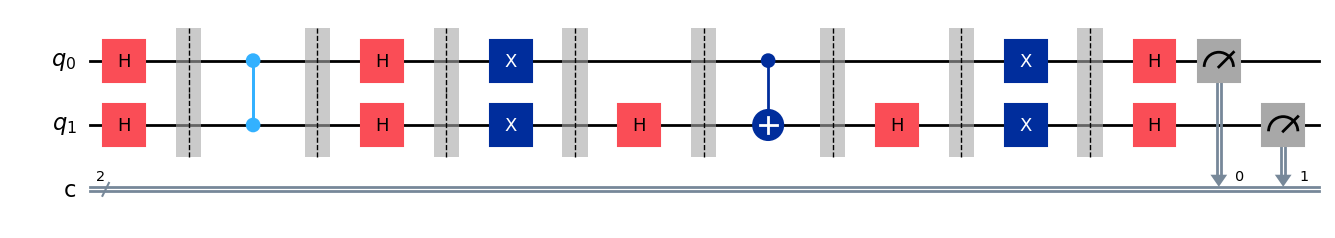
\includegraphics[width=1\textwidth]{images/circuit_es4.png}
    \caption{Qiskit circuit}
    \label{fig:circuit es4}
\end{figure}




%% Qasm 
\begin{lstlisting}[language=Python, caption={Export circuit to QASM3}, label={lst:qasm-export}]
qasm_str = dumps(qc)
print(qasm_str)
\end{lstlisting}

\begin{lstlisting}[language=Python, caption={Output generato: OpenQASM 3}, label={lst:qasm3-output}, backgroundcolor=\color{bg}]
OPENQASM 3.0;
include "stdgates.inc";
bit[2] c;
qubit[2] q;
h q[0];
h q[1];
barrier q[0], q[1];
cz q[1], q[0];
barrier q[0], q[1];
h q[0];
h q[1];
barrier q[0], q[1];
x q[0];
x q[1];
barrier q[0], q[1];
h q[1];
barrier q[0], q[1];
cx q[0], q[1];
barrier q[0], q[1];
h q[1];
barrier q[0], q[1];
x q[0];
x q[1];
barrier q[0], q[1];
h q[0];
h q[1];
c[0] = measure q[0];
c[1] = measure q[1];
\end{lstlisting}

\begin{figure}[H]
    \centering
    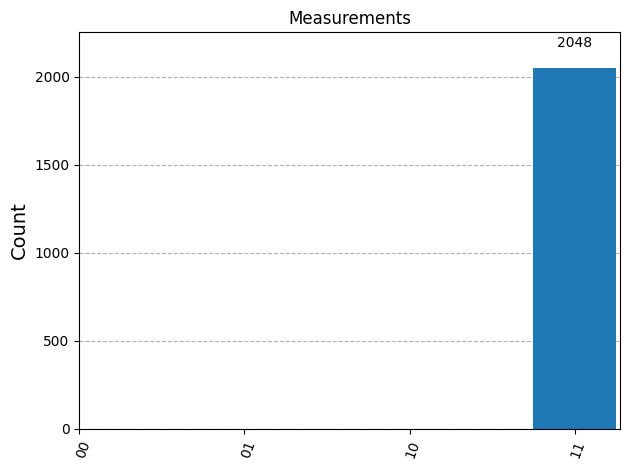
\includegraphics[width=0.7\textwidth]{images/histograms.png}
    \caption{output histogram}
    \label{fig:output histogram}
\end{figure}
